%\newpage
%============================================================================================================================


\chapter{Реализация графа в Coq}

\section{Представление графов в Coq}
Реализации графов из статьи де Грея приведены в файле {\tt myGraphs.v}~\ref{lst:myGraphs}
Эффективное представление графа было взято из\cite{VFA} и устроено
следующим образом: граф -- это конечное отображение, каждую вершину
(помеченную целым положительными числом) переводящее во
множество вершин с нею смежных. Конечные отображения и множества
формализованы с помощью модулей FSets и FMaps из стандартной
библиотеки. Эти модули принимают различные типы ключей, в данном случае мы будем использовать тип {\tt positive} целых положительных чисел в двоичном представлении из модуля {\tt PositiveOrderedTypeBits}.

\begin{verbatim}
Module E := PositiveOrderedTypeBits.
Module S <: FSetInterface.S := PositiveSet.
Module M <: FMapInterface.S := PositiveMap.
\end{verbatim} 

Вершина {\tt node} -- это элемент типа {\tt positive}, {\tt nodemap} -- это отображение из вершин, а граф {\tt graph} -- это отображение из типа вершина в тип множество вершин. Тип {\tt positive} был выбран из-за того, что в нем оператор сравнения определен так, чтобы поиск по ключу типа {\tt positive} в множестве и отображении был более эффективным.

\begin{verbatim}
Definition node := E.t.
Definition nodeset := S.t.
Definition nodemap: Type -> Type := M.t.
Definition graph := nodemap nodeset.
\end{verbatim}

Для работы с графами были определены функции добавления ребра в существующий граф и построения графа из списка ребер.

\begin{verbatim}
Definition add_edge (e: (E.t*E.t)) (g: graph) : graph :=
 M.add (fst e) (S.add (snd e) (adj g (fst e))) 
  (M.add (snd e) (S.add (fst e) (adj g (snd e))) g).
\end{verbatim}

В данной функции ребро представляется парой вершин.
В данной работе реализуются неориентированные графы без петель.

\begin{verbatim}
Definition mk_graph (el: list (E.t*E.t)) :=
  fold_right add_edge (M.empty _) el.
\end{verbatim}

В терминах определенных выше функций построение графа {\tt K3} выглядит следующим образом:
\begin{verbatim}
Definition K3 := 
    mk_graph [ (1, 2) ; (2, 3); (1, 3)].
\end{verbatim}

Далее для работы с графом можно использовать функцию вывода множества вершин и функцию {\tt gr\_show} вывода множества ребер.
\begin{verbatim}
Compute (S.elements (Mdomain K3)).
\end{verbatim}
{\it = [2; 1; 3]}

{\it    : list S.elt.}

\begin{verbatim}
Function gr_show (g : graph) : list (node * node) :=
  S.fold 
    (fun n l => (map (fun y => (n, y)) (S.elements (adj g n))) ++ l) 
    (Mdomain g) nil.
\end{verbatim}

\begin{verbatim}
Compute gr_show K3.
\end{verbatim}
{\it = [(3, 2); (3, 1); (1, 2); (1, 3); (2, 1); (2, 3)] }

{\it   : list (node * node) }

В статье \cite{deGrey} автор приводит граф единичных расстояний {\tt N}, который раскрашивается в 4 цвета. Этот граф строится поэтапно на основании других графов. Сначала автор рассматривает граф $$H := (\{1, 2, 3, 4, 5, 6, 7 \},$$
    $$ \{(1, 2), (1, 3), (1, 4), (1, 5), (1, 6), (1, 7), $$
    $$ (2, 3), (3, 4), (4, 5), (5, 6), (6, 7), (7, 2)\}) $$ и замечает, что существет 4 существенно различных способа правильно раскрасить граф {\tt H} в не более чем 4 цвета.
    
Далее автор поэтапно, через графы {\tt H}, {\tt J} и {\tt K}, строит граф {\tt L} и рассматривает его правильные раскраски.

Конструкции графов в работе де Грея обладают
высокой степенью симметрии. Мы разработали и частично верифицировали в
системе {\tt Coq} методы построения таких графов. Именно, мы реализуем
функцию {\tt mk\_art}, которая соединяет два графа по вершине, {\tt mk\_cmn\_edge}, которая соединяет два графа по ребру и {\tt add\_edges}, которая добавляет ребра в граф.

Для реализации этих функций потребовались следующие вспомогательные функции.
Рекурсивная функция {\tt l\_rng} находит минимум и максимум в списке, функция {\tt gr\_rng} находит в графе минимальный и максимальный номера вершин. Функция {\tt rename\_all} принимает на вход граф {\tt G} и функцию {\tt f} из номеров вершин в номера вершин и выдает граф, полученный применением {\tt f} к вершинам графа {\tt G}. Функция {\tt delete\_edge} удаляет ребро из графа, а функция {\tt rename\_in\_order} переименовывает вершины графа в отрезок от $1$ до количества вершин, сохраняя при этом их порядок.


В терминах описанных функций конструкция графа {\tt H} на основе графа {\tt K3} выглядит следующим образом:

\begin{verbatim}
Definition H : graph := 
  let g1 := rename_in_order (mk_cmn_edge K3 K3 1 3 1 3) in
  let g2 := rename_in_order 
                (mk_cmn_edge g1 K3 1 (snd (gr_rng g1)) 1 3) in
  let g3 := rename_in_order 
                (mk_cmn_edge g2 K3 1 (snd (gr_rng g2)) 1 3) in
  let g4 := rename_in_order 
                (mk_cmn_edge g3 K3 1 (snd (gr_rng g3)) 1 3) in
  rename_in_order (add_edge (2, snd (gr_rng g4)) g4).
\end{verbatim}

Т.~е. граф {\tt H} построен из $5$ копий {\tt K3}, склеенных друг с другом по ребру, и добавленного ребра.

\begin{figure}[ht] 
  \center
  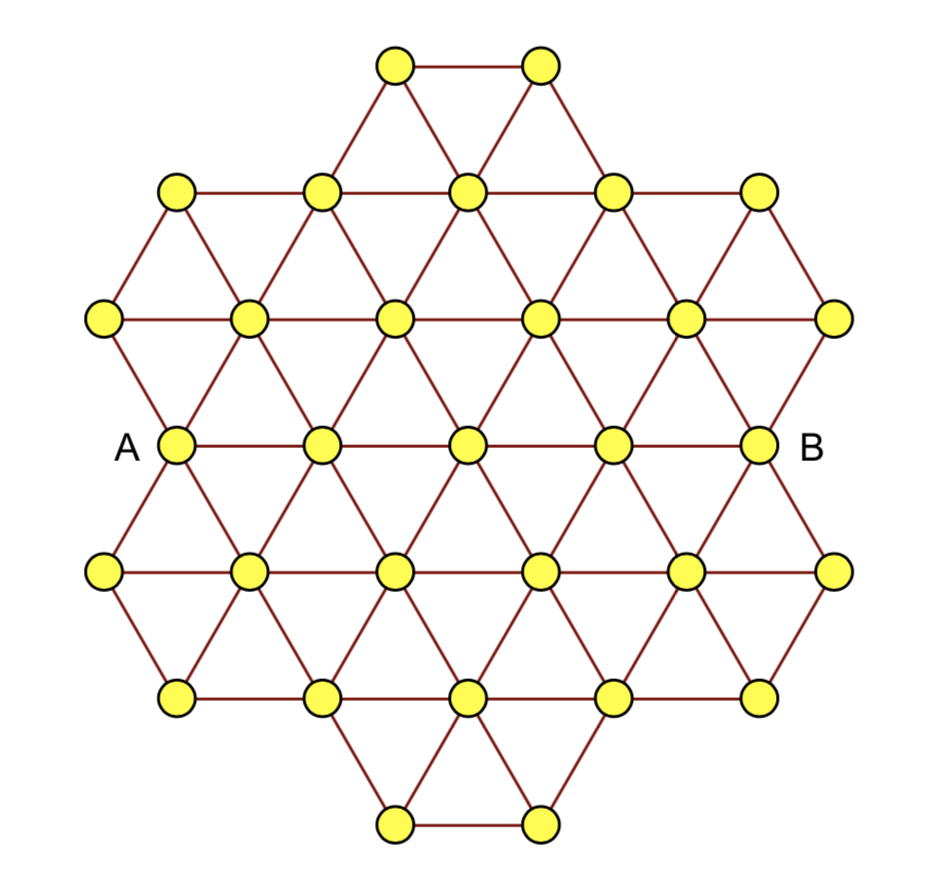
\includegraphics [width=0.5\linewidth] {Graph_J}
  \caption{Граф J} 
  \label{img:Graph_J}
\end{figure}

Граф {\tt J} состоит их 6 копий {\tt H}, склеенных между собой по ребру.
\begin{verbatim}
Definition J: graph :=
  let HH := mk_cmn_edge H H 2 3 6 7 in
  let HH_H := mk_cmn_edge HH H 7 2 6 7 in
  let HHH := rename_node 14 12 HH_H in
  let HHH_H := mk_cmn_edge HHH H 6 7 6 7 in
  let HHHH := rename_node 19 17 HHH_H in
  let HHHH_H := mk_cmn_edge HHHH H 5 6 6 7 in
  let HHHHH := rename_node 24 22 HHHH_H in
  let HHHHH_H := mk_cmn_edge HHHHH H 4 5 6 7 in
  let HHHHHH := rename_node 29 27 HHHHH_H in
  let HHHHHH_H := mk_cmn_edge HHHHHH H 3 4 6 7 in
  let HHHHHHH :=  rename_node 34 32 HHHHHH_H in
  rename_in_order (rename_node 37 9 HHHHHHH).
\end{verbatim}

В графе {\tt J} вершины, находящиеся на расстоянии $2$ от центра (в данной реализации вершины 9, 12, 16, 20, 24, 28) называются {\it соединяющими вершинами}.

\begin{figure}[ht] 
  \center
  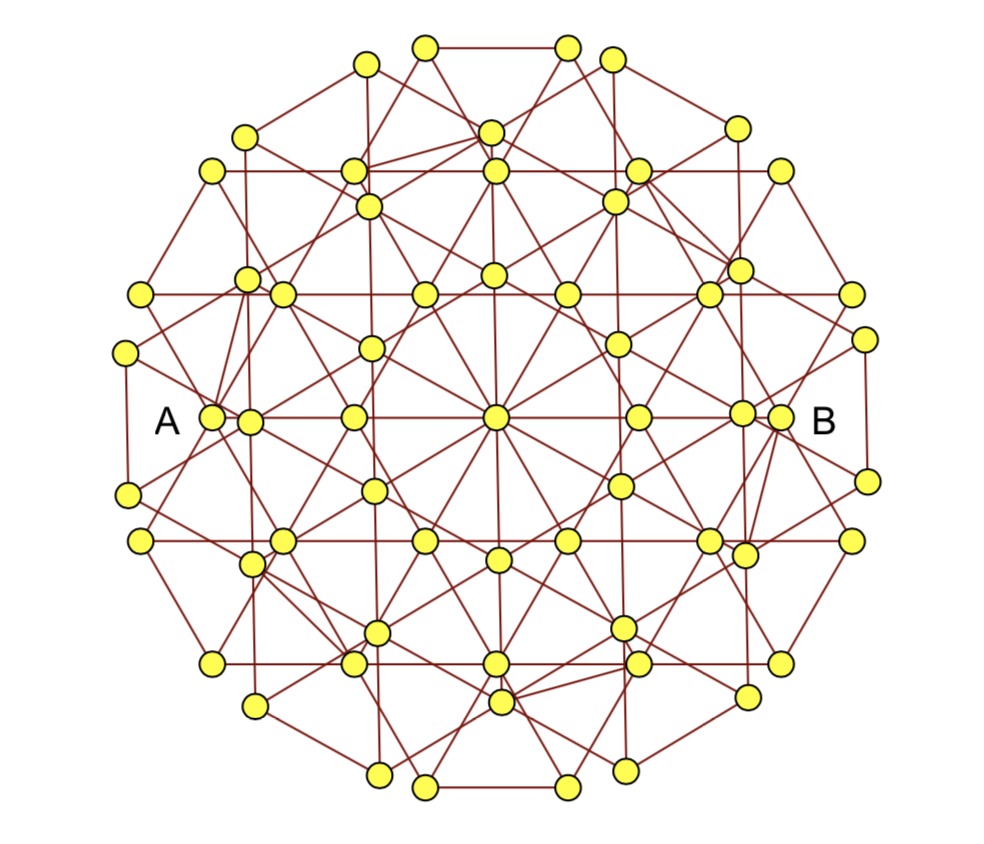
\includegraphics [width=0.8\linewidth] {Graph_K}
  \caption{Граф K} 
  \label{img:Graph_K}
\end{figure}

Граф {\tt K} состоит из двух копий графа {\tt J}, соединенных по центру, и ребер между соответствующими {\it соединяющими вершинами}.

\begin{verbatim}
Definition K: graph :=
  let JJ := mk_art J J 1 1 in
  let JJ := add_edges [
            (9, 9+31); (12, 12+31); (16, 16+31);
            (20, 20+31); (24, 24+31); (28, 28+31)] JJ in
  rename_in_order JJ.
\end{verbatim}

Наконец, граф {\tt L} состоит из двух копий графа {\tt K}, склееных между собой по {\it соединяющей вершине} и ребра между соединяющими вершинами, являющимися противоположными точке соединения.

\begin{figure}[ht] 
  \center
  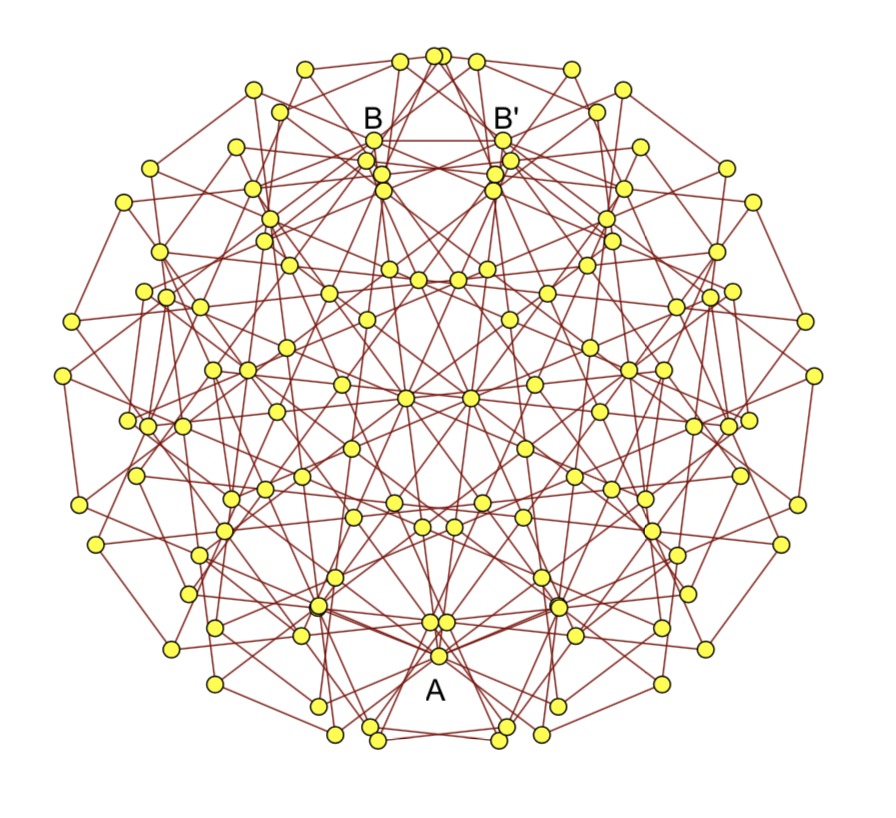
\includegraphics [width=0.8\linewidth] {Graph_L}
  \caption{Граф L} 
  \label{img:Graph_L}
\end{figure}

\section{Доказательства корректности операций над графами}

В файле {\tt myGraphs\_Properties.v}~\ref{lst:myGraphs_Properties} представлены доказательства корректности отпределенных ранее графов, т.~е. что они являются неориентированными графами без петель. 

\begin {verbatim}
Definition graph_ok (g : graph) := 
  undirected g /\ no_selfloop g.
\end{verbatim}

Для доказательства корректности графов введены и доказаны вспомогательные леммы {\tt adj\_M\_In} и {\tt edge\_corr\_1}.

\begin {verbatim}
Lemma adj_M_In : forall g n m,
  S.In m (adj g n) -> M.In n g.
\end{verbatim}

\begin {verbatim}
Lemma edge_corr_1 : forall g n m, edge g n m -> S.In m (nodes g).
\end{verbatim}

А также определена тактика {\tt gr\_destr}.

\begin {verbatim}
Ltac gr_destr h :=   apply S.elements_1 in h; compute in h;
  repeat rewrite InA_cons in h; rewrite InA_nil in h;
  repeat destruct h as [? | h]; try inversion h; subst.
\end{verbatim}

Данная тактика из посылки, что {\tt i} -- вершина графа, заключает, что {\tt i} равняется какому-то числу от $1$ до количества вершин и использует инверсию на этой посылке, тем самым перебирая все возможные вершины графа.

С использованием этой тактики доказательство корректности выглядит одинаково для любого построенного выше графа, приведем его для {\tt H}:

\begin{verbatim}
Lemma H_ok : graph_ok H.
Proof.
split.
- unfold undirected. intros. remember H as H'.
  clear HeqH'. apply edge_corr_1 in H.
  gr_destr H; gr_destr H';  reflexivity.
- unfold no_selfloop. repeat intro. remember H as H'.
  clear HeqH'. apply edge_corr_1 in H. gr_destr H; gr_destr H';
  discriminate.
Qed.
\end{verbatim}

Наряду с непосредственной проверкой корректности графов, можно доказать сохранение свойств отсутствия ориентации и петель нашими функциями, привлекаемыми для их построения (такими как {\tt add\_edge} и пр.). Очевидно, такой подход более универсален и более эффективен, поскольку, например уже для графа {\tt J} верификация доказательства занимает существенное время:

\begin{verbatim}
Lemma J_ok : graph_ok J.
Proof.
split.
- unfold undirected. intros. remember H as H'.
  clear HeqH'. apply edge_corr_1 in H.
  gr_destr H; gr_destr H';  reflexivity.
- unfold no_selfloop. repeat intro. remember H as H'.
  clear HeqH'. apply edge_corr_1 in H. gr_destr H; gr_destr H';
  discriminate.
Time Qed.
\end{verbatim}

{\it J\_ok is defined}

{\it Finished transaction in 73.252 secs (67.009u,0.208s) (successful) }

Мы приводим доказательство теоремы 

\begin{verbatim}
Lemma add_edge_corr : forall g a b, graph_ok g -> a <> b -> 
  graph_ok (add_edge (a, b) g).
\end{verbatim}
в файле {\tt myGraphs\_Properties.v}. Оно опирается на лемму 

\begin{verbatim}
Lemma add_edge_corr' : forall g x y a b,
  edge (add_edge (a, b) g) x y <-> edge g x y \/ (x = a /\ y = b) \/ 
  (x = b /\ y = a).
\end{verbatim}

дающую спецификацию функции {\tt add\_edge} и доказываемую с помощью принципа индукции {\tt WP.map\_induction} для конечных отображений из стандартной библиотеки.

\chapter{Доказательство свойств раскраски малых графов в Coq}
Назовем две раскраски $f$, $f'$ графа $G$ {\it существенно одинаковыми}, если существуют изоморфизм графа $g$ и перестановка цветов $ \omega $ такие, что
$f(v) = \omega ( f'( g(v) ) )$ . Также назовем две раскраски {\it существенно различными}, если они не являются существенно одинаковыми.

{\it Граф H} -- это граф $$H := (\{1, 2, 3, 4, 5, 6, 7 \},$$
    $$ \{(1, 2), (1, 3), (1, 4), (1, 5), (1, 6), (1, 7), $$
    $$ (2, 3), (3, 4), (4, 5), (5, 6), (6, 7), (7, 2)\}) $$
    

\begin{figure}[ht] 
  \center
  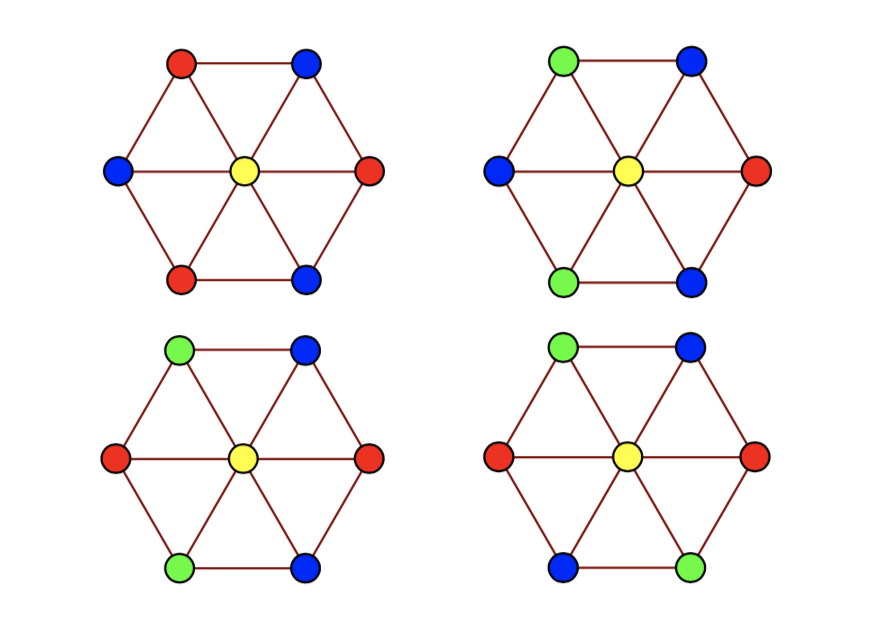
\includegraphics [width=0.8\linewidth] {Colorings_of_H}
  \caption{Существенно различные способы раскрасить граф H в не более чем 4 цвета} 
  \label{img:Colorings_of_H}
\end{figure}

В статье \cite{deGrey} утверждается что существует только 4 существенно различные раскраски графа {\tt H} в не более чем в 4 цвета. Это утверждение обосновывается перебором вариантов наличия или отсутствия монохроматических троек.

Описание типов для работы с раскрасками находятся в файле {\tt my\_New\_Coloring.v}~\ref{lst:my_New_Coloring}. В нем описан индуктивный предикат {\tt is\_color}, где {\tt is\_color} означает, что номер цвета содержится в палитре из 4 цветов. Тот факт, что этот тип индуктивный, позволяет использовать тактику {\tt inversion}, перебирая разрешенные цвета.

\section{Язык {\tt Ltac}, {\tt pattern matching} и {\tt goal matching} }
В данной главе активно используется язык {\tt Ltac} и инструмент {\tt goal matching}, представляемый этим языком.
Язык {\tt Ltac}, впервые представленный в статье <<A Tactic Language for the System {\tt Coq}>>~\cite{Del00}, предоставляет оператор соответствия ({\tt pattern matching}) не только для термов, но и для контекста доказательства ({\tt goal matching}), т.~е. цели и посылок. Данный оператор позволяет автоматизировать применение низкоуровневых тактик и значительно сократить длину доказательства.

\section{Типы возможных правильных раскрасок графа {\tt T} в не более чем 4 цвета}

Назовем {\it тройкой} любой граф, изоморфный графу {\it T} на четырех вершинах $$T = (\{1, 2, 3, 4\} , \{(1, 2), (1, 3), (1, 4) \} ).$$

{\it Утверждение}: Существует только три существенно различные раскраски графа $G$, если граф $G$ изоморфен $T$.

Код доказательства этого утверждения приведен в файле {\tt my\_Triple\_Coloring.v}~\ref{lst:my_Triple_Coloring}. 

В системе {\tt Coq} эти раскраски можно описать следующим образом:

\begin{verbatim}
(* Monochromatic *)
Definition type1_triple (el: list node) (c: Coloring) :=
  let center := nth 0 el 1 in
  let v1 := nth 1 el 1 in
  let v2 := nth 2 el 1 in
  let v3 := nth 3 el 1 in
  let c1 := c center in
  let c2 := c v1 in
  ~ (c1 = c2) /\ same_color c v1 v2 /\ same_color c v2 v3.

(* 2 and 1 *)
Definition type2_triple (el: list node) (c: Coloring) :=
  let center := nth 0 el 1 in
  let v1 := nth 1 el 1 in
  let v2 := nth 2 el 1 in
  let v3 := nth 3 el 1 in

  let c1 := c center in
  let c2 := c v1 in
  let c3 := c v2 in 
  let c4 := c v3 in
  ~ (c1 = c2) /\ ~ (c1 = c3) /\ ~ (c1 = c4) /\
    ( (c2 = c3 /\ ~ c2 = c4) \/ (c2 = c4 /\ ~ c2 = c3) \/ 
        (c3 = c4 /\ ~ c3 = c2) ).

(* All 3 different *)
Definition type3_triple (el: list node) (c: Coloring) :=
  let center := nth 0 el 1 in
  let v1 := nth 1 el 1 in
  let v2 := nth 2 el 1 in
  let v3 := nth 3 el 1 in

  let c1 := c center in
  let c2 := c v1 in
  let c3 := c v2 in 
  let c4 := c v3 in
  ~ (c1 = c2) /\ ~ (c1 = c3) /\ ~ (c1 = c4) /\
    (~ c2 = c3) /\ (~ c2 = c4) /\ (~ c3 = c4).
\end{verbatim}

Каждый предикат принимает на вход список вершин и раскраску, при этом первый элемент в списке -- номер вершины, соединенной со всеми остальными. Предикат {\tt type1\_triple} кодирует то, что все вершины, кроме первой одинакового цвета, при этом этот цвет отличен от цвета первой вершины. Предикат {\tt type2\_triple} кодирует то, что цвет первой вершины отличен от цвета остальных вершин, а среди остальных есть две одинакового цвета, который отличен от цвета оставшейся вершины. Предикат {\tt type3\_triple} кодирует случай, когда все 4 вершины имеют различный цвет.

Теорема {\tt coloring\_triple\_T} утверждает, что любая правильная раскраска графа {\tt T} является раскраской одного из этих типов. Ее доказательство включает в себя перебор всех возможных раскрасок, однако благодаря использованию языка {\tt Ltac} и {\tt goal matching} можно переиспользовать куски доказательства в ситуациях, отличающихся только перестановкой цветов или изоморфизма графа.

Тактика {\tt contr} доказывает {\tt coloring\_triple\_T} от противного и применяется в случаях, когда раскраска не является правильной, т.~е. существует пара смежных ребер одного цвета. Тактика {\tt type1\_tac} применяется, когда полученная раскраска является раскраской первого типа, тактики {\tt type1\_tac\_left}, {\tt type1\_tac\_middle}, {\tt type1\_tac\_right} -- раскраской второго типа (какая именно тактика будет применена зависит от того, какая пара вершин окрашена в один цвет) и тактика {\tt type3\_tac} применяется для доказательства того, что раскраска является раскраской третьего типа.

Таким образом, для любой раскраски графа {\tt T} существует тактика, с помощью которой можно доказать утверждение о том, что если раскраска правильная, то она является раскраской одного из трех типов. Теперь все эти тактики можно объединить в одну тактику {\tt level4}, которая с помощью {\tt goal matching} может определить, какую именно тактику из указанных использовать. Теперь можно создать тактики {\tt level3} и {\tt level2}, которые также с помощью {\tt goal matching} определяют, необходимо ли доказывать утверждение от противного или вызывать тактику следующего уровня.

Итак, благодаря {\tt goal matching} доказательство утверждения при различных контестах может быть доказано одной и той же тактикой, что позволяет использовать конвейер и записать доказательство теоремы очень кратко

\begin{verbatim}
Lemma coloring_triple_T:
  forall c: Coloring, is_good_coloring c T ->
  type1_triple [1; 2; 3; 4] c \/ type2_triple [1; 2; 3; 4] c \/
  type3_triple [1; 2; 3; 4] c.
Proof.
  intros. unfold is_good_coloring in H. unfold is_coloring in H. 
  destruct H. remember H as H'. clear HeqH'. 
  specialize (H' 1). inversion H';
    remember H as H''; clear HeqH''; specialize (H'' 2); 
    inversion H''; remember H0 as H0'; clear HeqH0';
      level2 H H0' H0 H2 H3 c.
Qed.
\end{verbatim}

\section{Типы возможных правильных раскрасок графа {\tt H} в не более чем 4 цвета}

Теперь, когда доказано утверждение про правильные раскраски {\it троек}, можно перейти к раскраскам графа {\it H}.

Типы раскрасок графа {\it H} в не более чем 4 цвета можно описать следующими предикатами в системе {\tt Coq}.

\begin{verbatim}
(* Type1 triple - Type1 triple *)
Definition type1_H (c: Coloring) : Prop :=
  type1_triple [1; 2; 4; 6] c /\ type1_triple [1; 3; 5; 7] c /\
    ~ same_color c 2 3.

(* Type1 triple - Type2 triple *)
Definition type2_H (c: Coloring) : Prop :=
  (type1_triple [1; 2; 4; 6] c /\ type2_triple [1; 3; 5; 7] c /\
    ~ same_color c 2 3 /\ ~ same_color c 2 5 /\ ~ same_color c 2 7) \/
  (type2_triple [1; 2; 4; 6] c /\ type1_triple [1; 3; 5; 7] c /\
    ~ same_color c 2 3 /\ ~ same_color c 4 3 /\ ~ same_color c 6 3).

(* Diagonals are monochromatic *)
Definition type3_H (c: Coloring) : Prop :=
  type3_triple [1; 2; 4; 6] c /\ type3_triple [1; 3; 5; 7] c /\
    same_color c 2 5 /\ same_color c 3 6 /\ same_color c 4 7.

(* One monochromatic diagonal and 
same colors close to the vertices in diagonal *)
Definition type4_H (c: Coloring) : Prop :=
  type2_triple [1; 2; 4; 6] c /\ type2_triple [1; 3; 5; 7] c /\
  (
    (* Diagonal is 2 5 *) 
    (same_color c 2 5 /\ same_color c 3 7 /\ same_color c 4 6 ) \/

    (* Diagonal is 3 6 *) 
    (same_color c 3 6 /\ same_color c 2 4 /\ same_color c 5 7 ) \/

    (* Diagonal is 4 7 *) 
    (same_color c 4 7 /\ same_color c 3 5 /\ same_color c 2 6 )
  ).
\end{verbatim}

В системе {\tt Coq} теорема о возможных раскрасках графа {\tt H} формулируется следующим образом:

\begin{verbatim}
Lemma coloring_H:
  forall c: Coloring, is_good_coloring c H ->
  type1_H c \/ type2_H c \/ type3_H c \/ type4_H c.
\end{verbatim}

Полный код доказательства находится в файле {\tt my\_H\_Coloring.v}~\ref{lst:my_H_coloring}.

Как и в предыдущем разделе, можно определить тактику {\tt contr}, которая доказывает утверждение от противного, т.~е. доказывает, что данная раскраска не является правильной. Но так как теперь вершин в графе больше и не всегда понятно, какие именно смежные вершины окрашены в одинаковый цвет, доказательство упрощает использование тактики {\tt find\_contr}, которая перебирает гипотезы-посылки о том, что какие-то две вершины покрашены в один цвет в контексте доказательства и пытается из этих гипотез вывести, что раскраска не является правильной. 

Также определены тактики 

{\tt type1\_H\_tac}, {\tt type2\_H\_tac\_left\_left}, {\tt type2\_H\_tac\_left\_right}, {\tt type2\_H\_tac\_left\_middle}, {\tt type2\_H\_tac\_right\_left}, {\tt type2\_H\_tac\_right\_middle}, {\tt type2\_H\_tac\_right\_right}, {\tt type3\_H\_tac}, {\tt type4\_H\_tac\_1}, {\tt type4\_H\_tac\_2}, {\tt type4\_H\_tac\_3} для каждого подтипа раскраски. Для автоматизации использования этих тактик разработана еще одна тактика {\tt find\_type}, в которой используется оператор соответствия цели ({\tt goal matching}). Тактика {\tt color\_next} <<окрашивает следующую вершину>>, т.~е. выводит посылку о том, что цвет следующей вершины принадлежит индуктивному типу {\tt is\_color} и делает инверсию этого типа.

Итоговое доказательство теоремы выглядит следующим образом:

\begin{verbatim}
Lemma coloring_H:
  forall c: Coloring, is_good_coloring c H ->
  type1_H c \/ type2_H c \/ type3_H c \/ type4_H c.
Proof.
  intros. unfold is_good_coloring in H. 
  unfold is_coloring in H. destruct H.
  color_next H 1;
    color_next H 2; try find_contr H0 c;
      color_next H 3; try find_contr H0 c;
        color_next H 4; try find_contr H0 c;
          color_next H 5; try find_contr H0 c;
            color_next H 6; try find_contr H0 c;
              color_next H 7; try find_contr H0 c;
                find_type H3 H5 H7 H9 H11 H13 H15 c.
Qed.
\end{verbatim}

\chapter{Работа в графами на {\tt Python}}
\section{Реализация графов на плоскости}
Все встречавшиеся ранее графы являются {\it графами единичных расстояний}, т.~е. существует такая реализация этих графов на плоскости, в которой каждое ребро имеет длину 1.

Работа с реализацией графа на плоскости в системе {\tt Coq} представляет затруднения, так как формализация представления и разработка операций над алгебраическими числами влечет за собой большую работу.

Чтобы получить реализацию графов на плоскости, использовался язык {\tt Python} и пакет для символьной математики {\tt Sympy}.

Код для генерации реализаций рассматриваемых графов на плоскости находится в файле {\tt SymPy\_Realization.py}.

Для работы с реализациями графов были определены следующие функции. Функция {\tt neg(pt)} отражает вектор {\tt pt} относительно начала координат, функция {\tt shifted(pt, vec)} сдвигает вектор {\tt pt} на вектор {\tt vec}, функция {\tt rotated(pt, angle)} поворачивает вектор {\tt pt} на угол {\tt angle} относительно начала координа, функция {\tt rotatedabout(pt, origin, angle)} поворачивает вектор {\tt pt} на угол {\tt angle} относительно точки {\tt origin}.

Генерация реализаций на плоскости графов {\tt H} и {\tt J} выглядят следующим образом:

\begin{verbatim}
def build_H():
    o = (Rational(0), Rational(0))
    e = (Rational(1), Rational(0))

    H = {o}
    for i in range(6):
        H.add(rotatedabout(e, o, pi / 3 * i))
    H = simplified(H)
    return H
\end{verbatim}

\begin{verbatim}
def build_J():
    J = {o}
    for i in range(6):
        J.update(
            { rotated(
                shifted(x, shifted(
                            e, rotated(e, pi / 3)
                                  ) 
                        ),
                pi / 3 * i) for x in H }
                )
    return simplified(J)
\end{verbatim}

Остальные графы вплоть до {\tt L} генерируются, как указано в статье~\cite{deGrey}.
% def dist2(p, q):
% def simplified(pts):
% def factored(pts):
% def check_zero(x):

\section{Алгоритм раскраски графов}
Одна из подзадач статьи~\cite{deGrey} заключается в том, чтобы найти такой граф {\tt M}, содержащий копию {\tt H}, что ни при какой правильной раскраске графа {\tt M} содержащаяся копия {\tt H} не содержит граф T', изоморфный T, раскрашенный по типу 1 (все три висячие вершины одного цвета).
В разделе 4 статьи~\cite{deGrey} предложен алгоритм для проверки графов на обладание указанным свойством.

Алгоритм обходит граф в глубину и красит встречающиеся вершины в первый доступный цвет. Если на каком-то шаге алгоритма есть вершина, для которой никакой цвет не является доступным, происходит {\it возврат} ({\tt backtracking}). А если на каком-то шаге есть вершины, для которых доступен только один цвет, то красятся эти вершины. Полный код алгоритма представлен в файле {\tt Color\_graph-M.py}.


\chapter{Заключение}
\section{Выводы}
В статье ~\cite{deGrey} представлен граф единичных расстояний {\tt N}, который не красится в 4 цвета. Этот граф представляет собой прямое произведение графов {\tt L} и {\tt M}.

В данной работе представлены эффективные методы конструирования графов, обладающих высокой степенью симметрии. Эти методы были применены к графам {\tt H}, {\tt J}, {\tt K} и {\tt L}.

Также разработаны методы работы с раскрасками графов и методики верифицирования доказательств теорем о свойствах раскрасок. Верифицировано доказательство того, что существует ровно 4 существенно различных раскрасок графа {\tt H}. Разработанные методы можно использовать и для других графов.

Графы из второй части статьи ~\cite{deGrey} реализованы не были в силу того, что их конструкция сильно опирается на реализацию этиз графов на плоскости. В то же время, был реализован на Python алгоритм из второй части статьи, с помощью которого производился поиск подходящего графа {\tt M}.

\section{Планы будущей работы}
Разработанные методы конструкции графов, обладающих высокой степенью симметрии, можно использовать для графов из статьи Marijn~J.H.~Heule, <<Computing Small Unit-Distance Graphs with Chromatic Number 5>>~\cite{Huele}, в которой приводится граф меньшего размера, который не красится в 4 цвета.

Методы работы в системе {\tt Coq} с раскрасками графов можно применить для доказательства свойств раскраски графов {\tt J}, {\tt K} и {\tt L}.

Также интерес представляет верифицирование с помощью {\Coq} алгоритма покраски графа из статьи~\cite{deGrey}, с помощью которого был осуществлен поиск графа, подходящего на роль {\tt M}.

\chapter{Приложение}

\begingroup
    \lstinputlisting[caption={Листинг myGraphs.v},label={lst:myGraphs}]{listings/myGraphs.v}
\endgroup
 
\begingroup
    \lstinputlisting[caption={Листинг myGraphs\_Properties.v},label={lst:myGraphs_Properties}]{listings/myGraphs_Properties.v}
\endgroup

\begingroup
    \lstinputlisting[caption={Листинг my\_New\_Coloring.v},label={lst:my_New_Coloring}]{listings/my_New_Coloring.v}
\endgroup


\begingroup
    \lstinputlisting[caption={Листинг my\_Triple\_Coloring.v},label={lst:my_Triple_Coloring}]{listings/my_Triple_Coloring.v}
\endgroup


\begingroup
    \lstinputlisting[caption={Листинг my\_H\_coloring.v},label={lst:my_H_coloring}]{listings/my_H_coloring.v}
\endgroup
 
\begingroup
    \lstinputlisting[caption={Листинг Color\_graph-M.py},label={lst:Color_graph-M},language={python}]{listings/Color_graph-M.py}
\endgroup
   
\begingroup
    \lstinputlisting[caption={Листинг SymPy\_Realization.py},label={lst:SymPy_Realization},language={python}]{listings/SymPy_Realization.py}
\endgroup

\label{chapt1}
